\section{Software in the Loop}

\subsection{Monte-Carlo}

\section{Hardware in the Loop}

\clearpage
\section{Testflight}
The Testflight launch was conducted on May 10th 2025 near Louisville, Kentucky.
The resulting state estimation data is shown in Figure \ref{fig:testflight}.

Due to an error with internal logging only the telemetry data is available. This data was transmitted by the Processor Board to the rocket CAN bus, sent over radio telemetry, and logged by the ground station computer.
Due to the telemetry bandwidth and lossy connection, data points are not recorded at high speeds and regular intervals, and in some cases bits were dropped resulting in larger jumps of the data (e.g. at about $t=8\mathrm{s}$, the altitude jumps from 250m to 512m instead of 256m).   

Due to a safety lockout triggered by a timer, the canard was commanded to zero for the entirety of the flight.
Therefore the rocket had no control authority, and some misalignment of the canards and fin cant led to a slow roll rate with a peak of about 2 rad/s, as can be seen in Figure \ref{fig:testflight-w}.

The rocket lifts off at about $t=8\mathrm{s}$, and reaches apogee at about $t=28\mathrm{s}$.
At $t=31\mathrm{s}$ the recovery system is deployed, at which point the mission of the Controls subsystem ends. 
After recovery deployment the state estimation becomes unreliable, as descent under parachutes is not modelled.

Overall the Estimator performed well, as simulations line up with actual flight. 

\begin{figure}[ht]
    \centering   
    \begin{subfigure}{0.49\textwidth}
        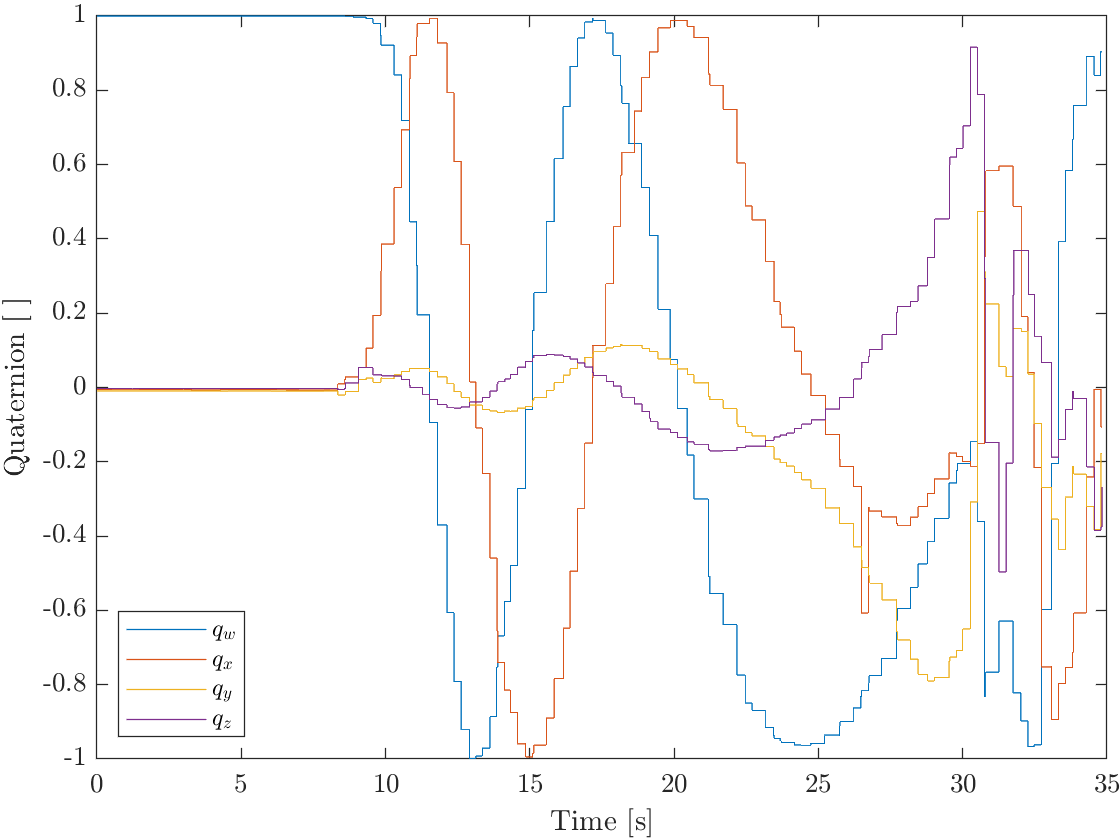
\includegraphics[width=0.95\textwidth]{images-results/testflight_q.png}
        \caption{Attitude Quaternion}
        \label{fig:testflight-q}
    \end{subfigure}
    \begin{subfigure}{0.49\textwidth}
        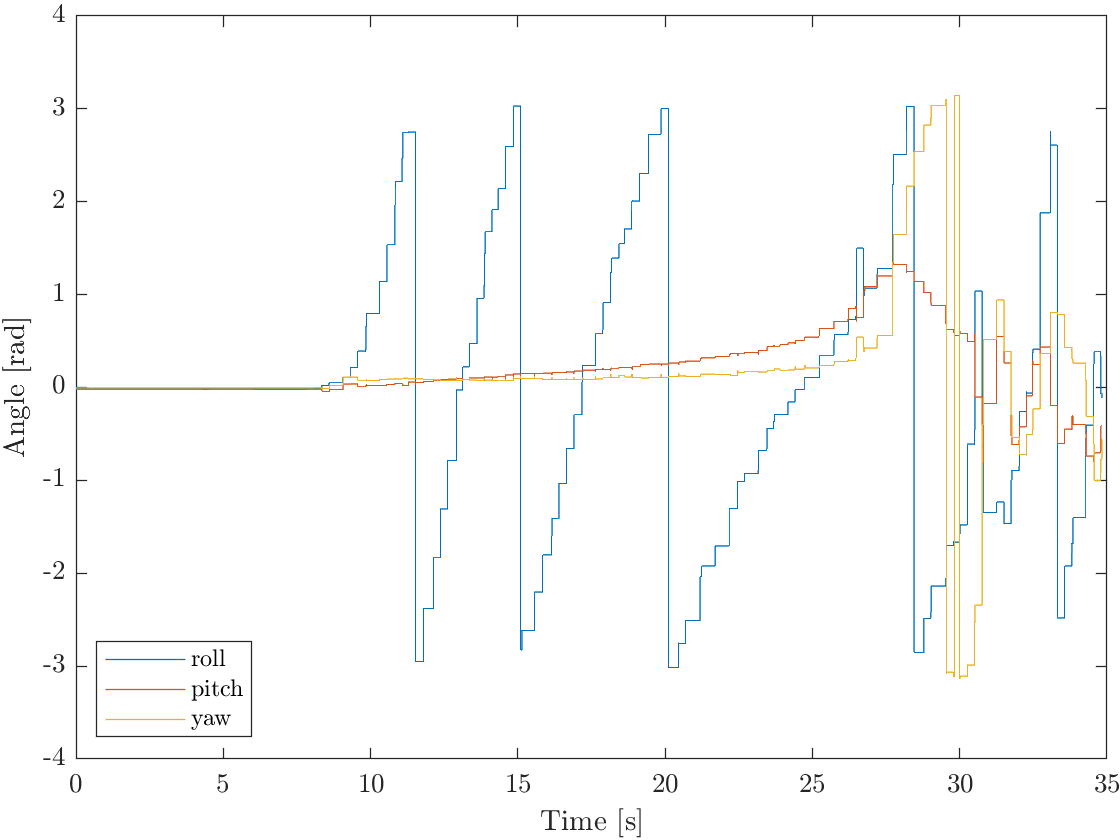
\includegraphics[width=0.95\textwidth]{images-results/testflight_euler.png}
        \caption{Attitude Euler angles}
        \label{fig:testflight-euler}
    \end{subfigure}
    \begin{subfigure}{0.49\textwidth}
        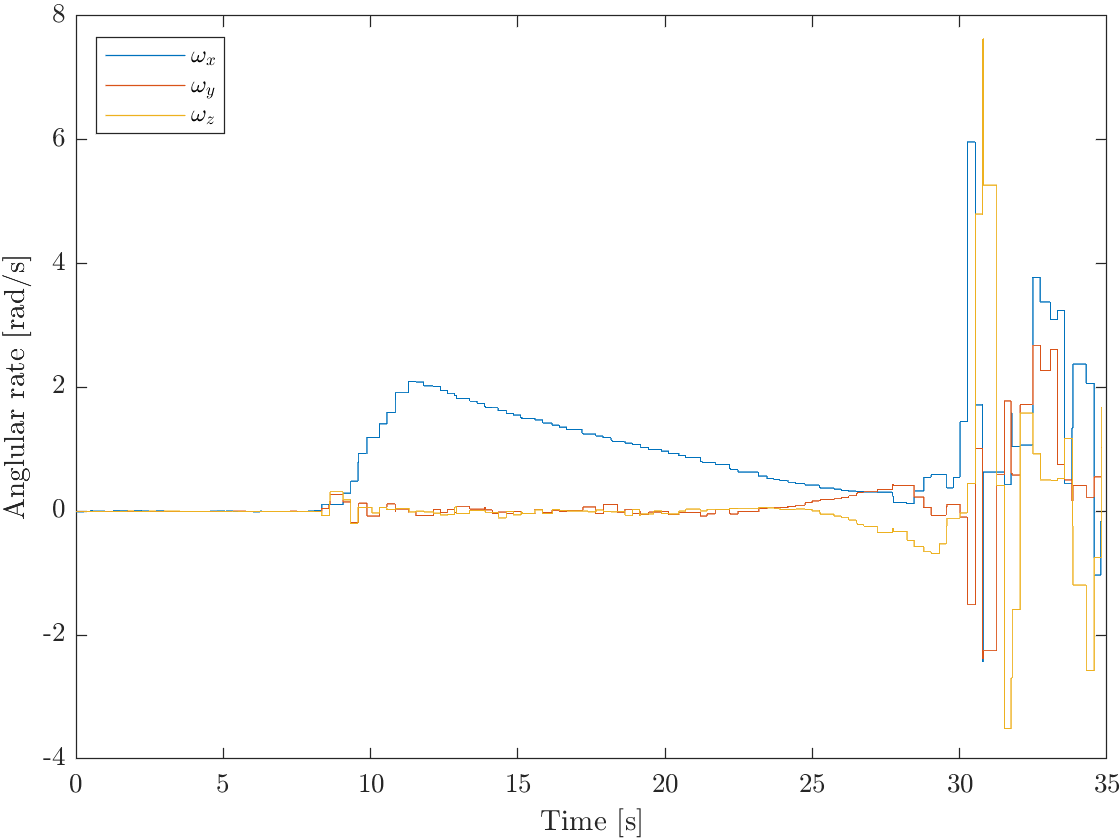
\includegraphics[width=0.95\textwidth]{images-results/testflight_w.png}
        \caption{Angular rates}
        \label{fig:testflight-w}
    \end{subfigure}
    \begin{subfigure}{0.49\textwidth}
        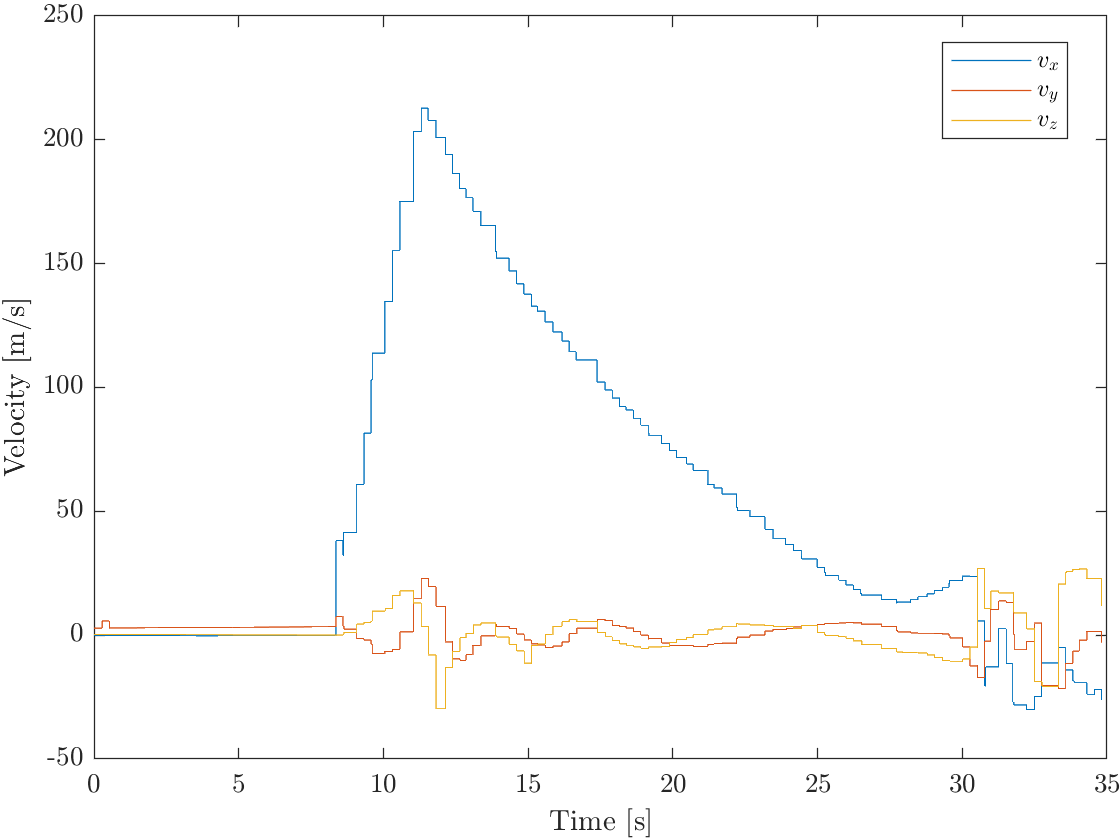
\includegraphics[width=0.95\textwidth]{images-results/testflight_v.png}
        \caption{Body velocity}
        \label{fig:testflight-v}
    \end{subfigure}
    \begin{subfigure}{0.49\textwidth}
        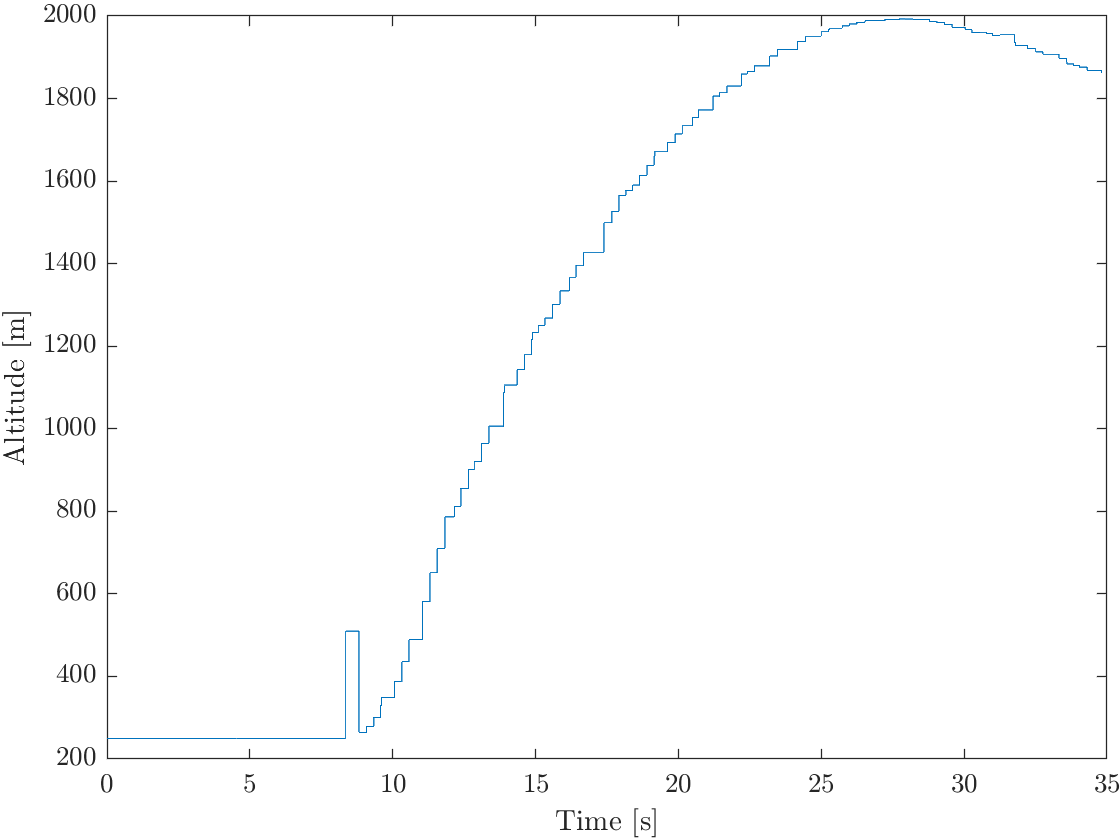
\includegraphics[width=0.95\textwidth]{images-results/testflight_alt.png}
        \caption{Altitude}
        \label{fig:testflight-alt}
    \end{subfigure}
    \begin{subfigure}{0.49\textwidth}
        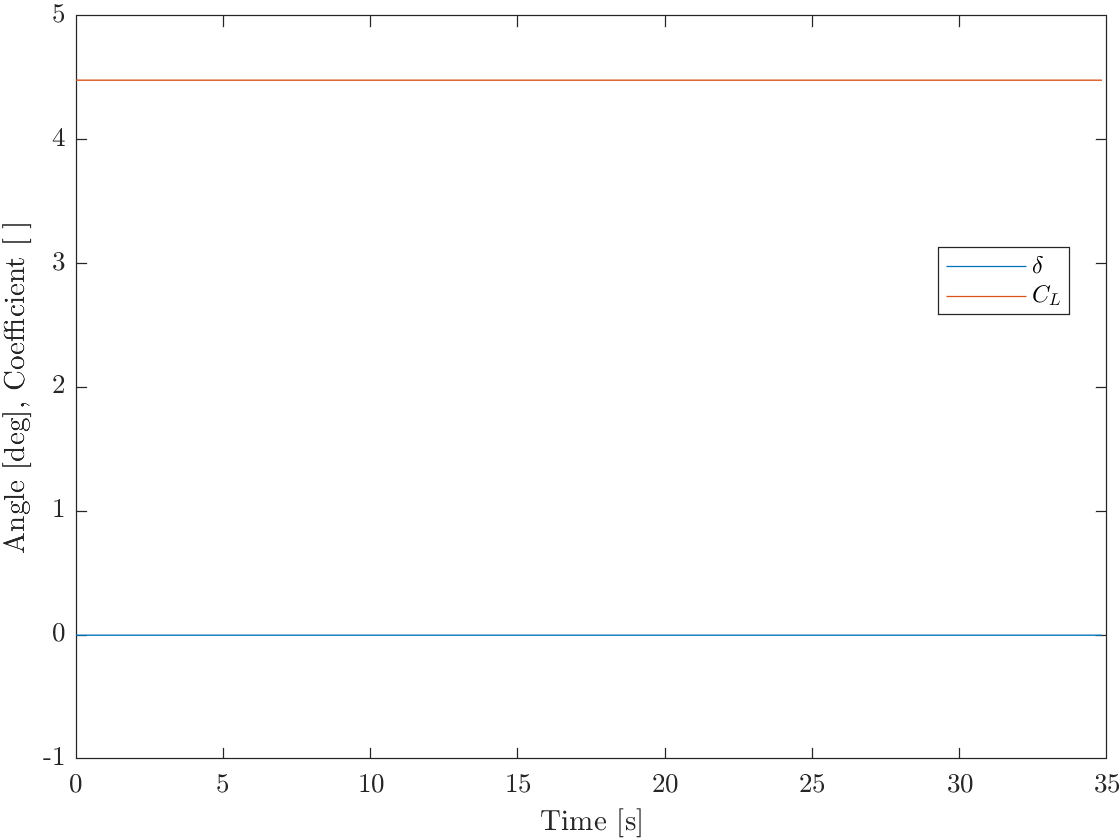
\includegraphics[width=0.95\textwidth]{images-results/testflight_canard.png}
        \caption{Canard}
        \label{fig:testflight-canard}
    \end{subfigure}
    \caption{Testflight telemetry, estimated state}
    \label{fig:testflight}
\end{figure}

\clearpage
\section{Competition flight}
